\section{Computational results}
\label{sec:results}

The finite calculations satisfy the stated identities and invariance checks. The tables report exact enumerations, and the figures display the corresponding results for the multiplicity and refinement families.

\subsection{Base models and Boolean extension}

The injective base contains six latent states and six reachable observations. Every fiber has size one, the observation map is injective, and an exact decoder exists. The noninjective comparison contains six latent states and three reachable observations. Each reachable fiber has size two, the model contains three unordered latent collisions, and no exact decoder exists. The Boolean extension contains twelve latent states and the same six reachable observations as the injective base. Its maximum fiber size is two, it contains six collision pairs, and no exact decoder exists.

\begin{table}[tbp]
\centering
\caption{Base and Boolean extension calculations.}
\label{tab:baseboolean}
\small
\begin{tabular}{@{}lrrrrcc@{}}
\toprule
Model & Latent & Reachable & Max. fiber & Collisions & Injective & Exact decoder \\
\midrule
Injective base & 6 & 6 & 1 & 0 & True & True \\
Noninjective base & 6 & 3 & 2 & 3 & False & False \\
Boolean extension & 12 & 6 & 2 & 6 & False & False \\
\bottomrule
\end{tabular}
\end{table}

\subsection{Finite hidden multiplicity}

The latent state count increases linearly with hidden multiplicity. The reachable observation count remains fixed at six, and the maximum fiber size equals the hidden multiplicity. The four panels show the latent-state, reachable-observation, fiber-size, and experiment-outcome consequences of the same multiplicity construction.

\begin{figure}[tbp]
\centering
\begin{subfigure}[t]{0.49\textwidth}
\centering
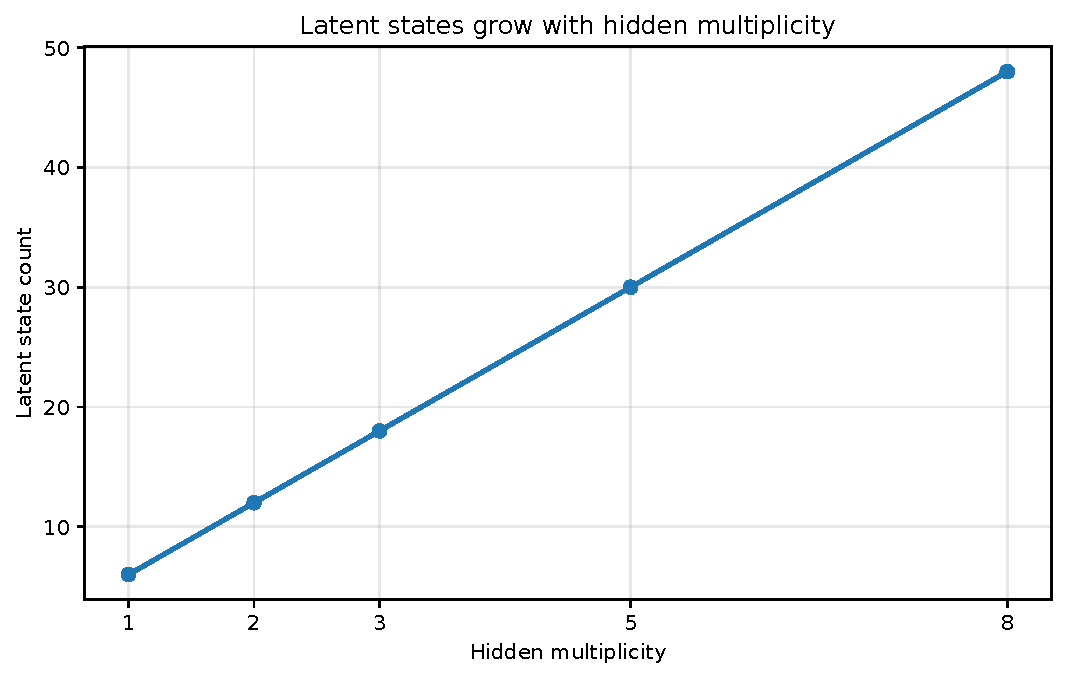
\includegraphics[width=\linewidth]{figures/repo_latent_state_count_vs_hidden_multiplicity.pdf}
\caption{Latent state count.}
\label{fig:repo-latent}
\end{subfigure}\hfill
\begin{subfigure}[t]{0.49\textwidth}
\centering
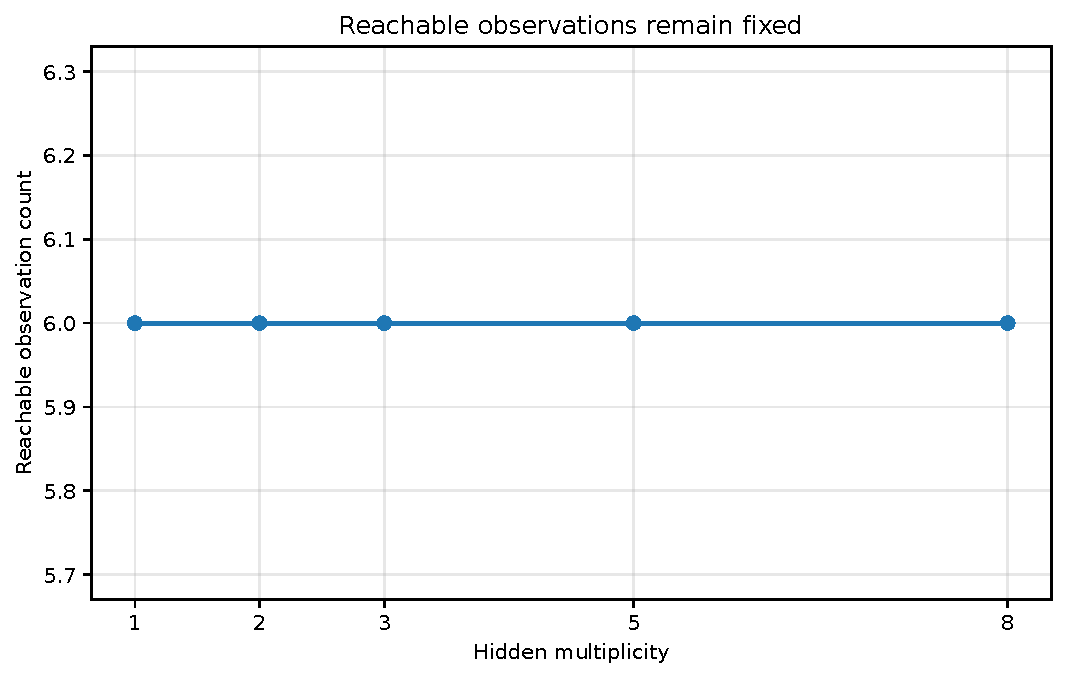
\includegraphics[width=\linewidth]{figures/repo_reachable_observation_count_vs_hidden_multiplicity.pdf}
\caption{Reachable observation count.}
\label{fig:repo-reachable}
\end{subfigure}

\vspace{0.6em}
\begin{subfigure}[t]{0.49\textwidth}
\centering
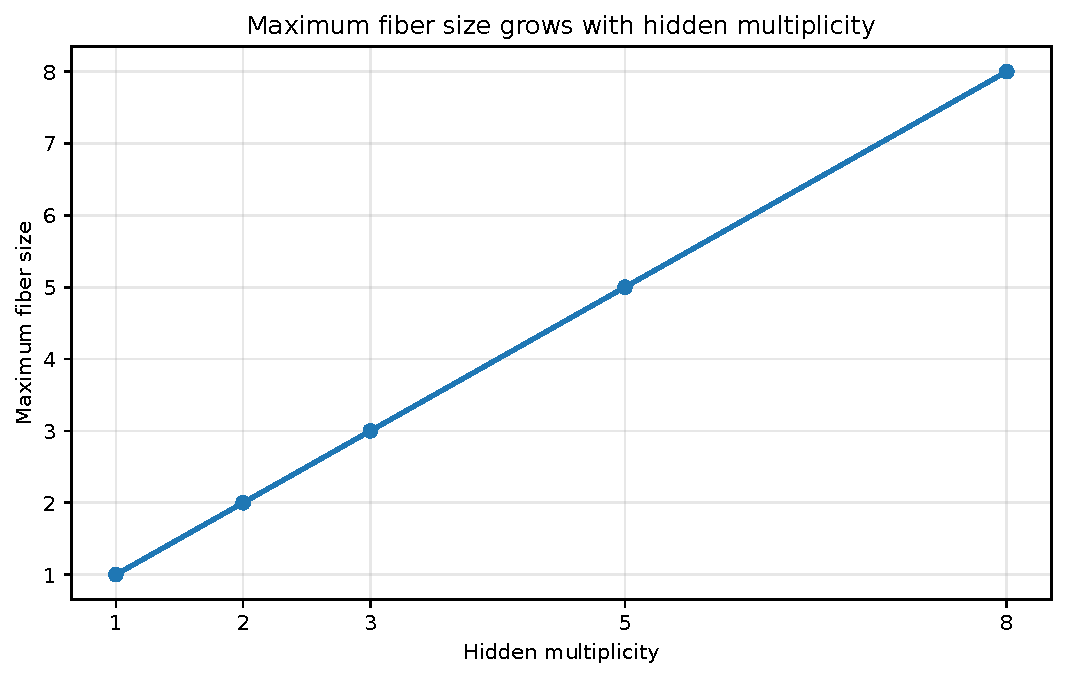
\includegraphics[width=\linewidth]{figures/repo_maximum_fiber_size_vs_hidden_multiplicity.pdf}
\caption{Maximum fiber size.}
\label{fig:repo-fiber}
\end{subfigure}\hfill
\begin{subfigure}[t]{0.49\textwidth}
\centering
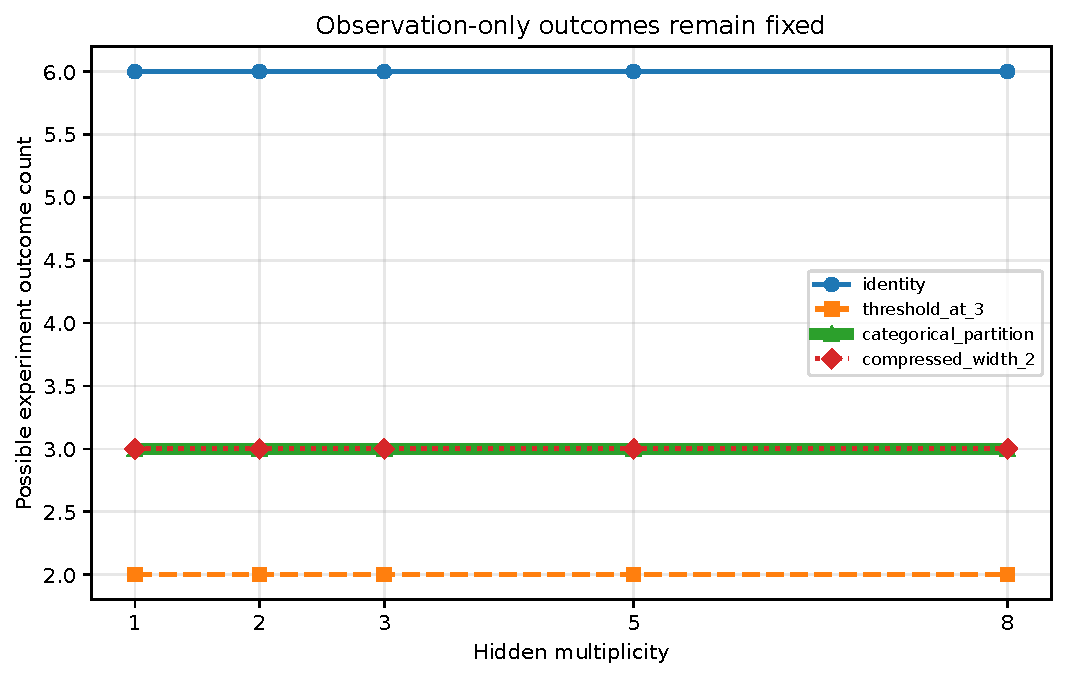
\includegraphics[width=\linewidth]{figures/repo_experiment_outcome_count_vs_hidden_multiplicity.pdf}
\caption{Observation only outcome counts.}
\label{fig:repo-experiments}
\end{subfigure}
\caption{Hidden multiplicity and observation only experiment results. The latent representation and observation fibers grow while the reachable observation set and each experiment's possible outcome count remain fixed.}
\label{fig:multiplicitypanel}
\end{figure}

\begin{table}[tbp]
\centering
\caption{Complete finite multiplicity summary.}
\label{tab:multiplicity}
\small
\begin{tabular}{@{}rrrrrrl@{}}
\toprule
\(m\) & Latent & Reachable & Avg. fiber & Max. fiber & Collisions & Exact decoder \\
\midrule
1 & 6 & 6 & 1.00 & 1 & 0 & True \\
2 & 12 & 6 & 2.00 & 2 & 6 & False \\
3 & 18 & 6 & 3.00 & 3 & 18 & False \\
5 & 30 & 6 & 5.00 & 5 & 60 & False \\
8 & 48 & 6 & 8.00 & 8 & 168 & False \\
\bottomrule
\end{tabular}
\end{table}

Every row is marked empirically equivalent to the base. Latent cardinality, fiber size, collision count, injectivity, and exact decoder status change while the reachable observation set remains fixed.

\subsection{Observation only experiments and predicate profiles}

The identity experiment has six possible outcomes. The threshold experiment has two. The categorical partition and width two compression experiments each have three. All twenty eight model and experiment comparisons match the base outcome set for the corresponding experiment.

\begin{table}[tbp]
\centering
\caption{Observation only outcome sets.}
\label{tab:experiments}
\small
\begin{tabularx}{\textwidth}{@{}lXcc@{}}
\toprule
Experiment & Possible outcomes & Count & All listed models match base \\
\midrule
Identity & \(\{0,1,2,3,4,5\}\) & 6 & True \\
Threshold at three & \(\{\mathrm{false},\mathrm{true}\}\) & 2 & True \\
Categorical partition & \(\{\mathrm{high},\mathrm{low},\mathrm{middle}\}\) & 3 & True \\
Compression width two & \(\{0,1,2\}\) & 3 & True \\
\bottomrule
\end{tabularx}
\end{table}

Three predicates are evaluated for seven model representations. All twenty one existential comparisons match the base success profile. All twenty one complete truth profile comparisons also match the base.

\begin{table}[tbp]
\centering
\caption{Base predicate profiles and comparison counts.}
\label{tab:predicates}
\small
\begin{tabularx}{\textwidth}{@{}lXcc@{}}
\toprule
Predicate & Base truth table on \(0,\ldots,5\) & Models compared & Matches \\
\midrule
Even & T, F, T, F, T, F & 7 & 7 \\
At least three & F, F, F, T, T, T & 7 & 7 \\
Endpoint \(\{0,5\}\) & T, F, F, F, F, T & 7 & 7 \\
\bottomrule
\end{tabularx}
\end{table}

\subsection{Finite empirical quotient and varying latent properties}

The finite grouping procedure produces two empirical classes. The first contains the injective base, Boolean extension, and finite multiplicity extensions. Its reachable set is \(\{0,1,2,3,4,5\}\), while its representatives have latent cardinalities \(6,12,18,30,48\). The second contains the noninjective comparison model with reachable set \(\{0,1,2\}\).

\begin{table}[tbp]
\centering
\caption{Finite empirical quotient.}
\label{tab:empiricalclasses}
\small
\begin{tabularx}{\textwidth}{@{}cXlX@{}}
\toprule
Class & Reachable observation set & Latent cardinalities & Representative types \\
\midrule
1 & \(\{0,1,2,3,4,5\}\) & 6, 12, 18, 30, 48 & Base, Boolean, and finite multiplicity extensions \\
2 & \(\{0,1,2\}\) & 6 & Noninjective comparison model \\
\bottomrule
\end{tabularx}
\end{table}

Four latent properties vary between the injective base and its Boolean extension although the two models occupy the same finite empirical class.

\begin{table}[tbp]
\centering
\caption{Properties that vary inside one finite empirical class.}
\label{tab:nonidentifiable}
\small
\begin{tabularx}{\textwidth}{@{}Xccc@{}}
\toprule
Property & Base & Boolean extension & Varies \\
\midrule
Latent cardinality & 6 & 12 & True \\
Maximum observation fiber size & 1 & 2 & True \\
Existence of exact latent decoder & True & False & True \\
Presence of Boolean hidden factor & False & True & True \\
\bottomrule
\end{tabularx}
\end{table}



\subsection{Interface refinement and quotient maps}

The identity and relabeled identity interfaces retain eight observable classes. Paired buckets retain four. Binary regions retain two. The strict refinements collapse four, eight, and twelve world state pairs. Their quotient maps are surjective and noninjective, and no reverse refinement exists. The relabeling maps collapse no pairs and induce bijections.

\begin{figure}[tbp]
\centering
\begin{subfigure}[t]{0.49\textwidth}
\centering
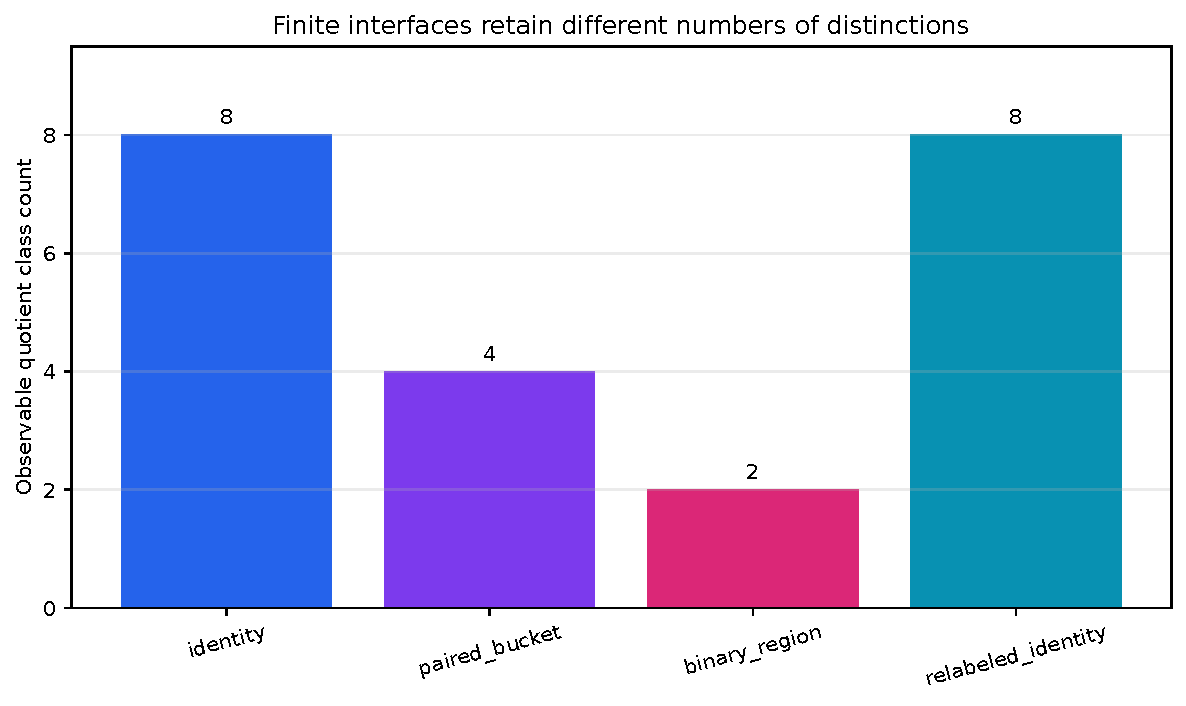
\includegraphics[width=\linewidth]{figures/repo_observable_quotient_size_by_interface.pdf}
\caption{Observable quotient size.}
\label{fig:repo-quotientsize}
\end{subfigure}\hfill
\begin{subfigure}[t]{0.49\textwidth}
\centering
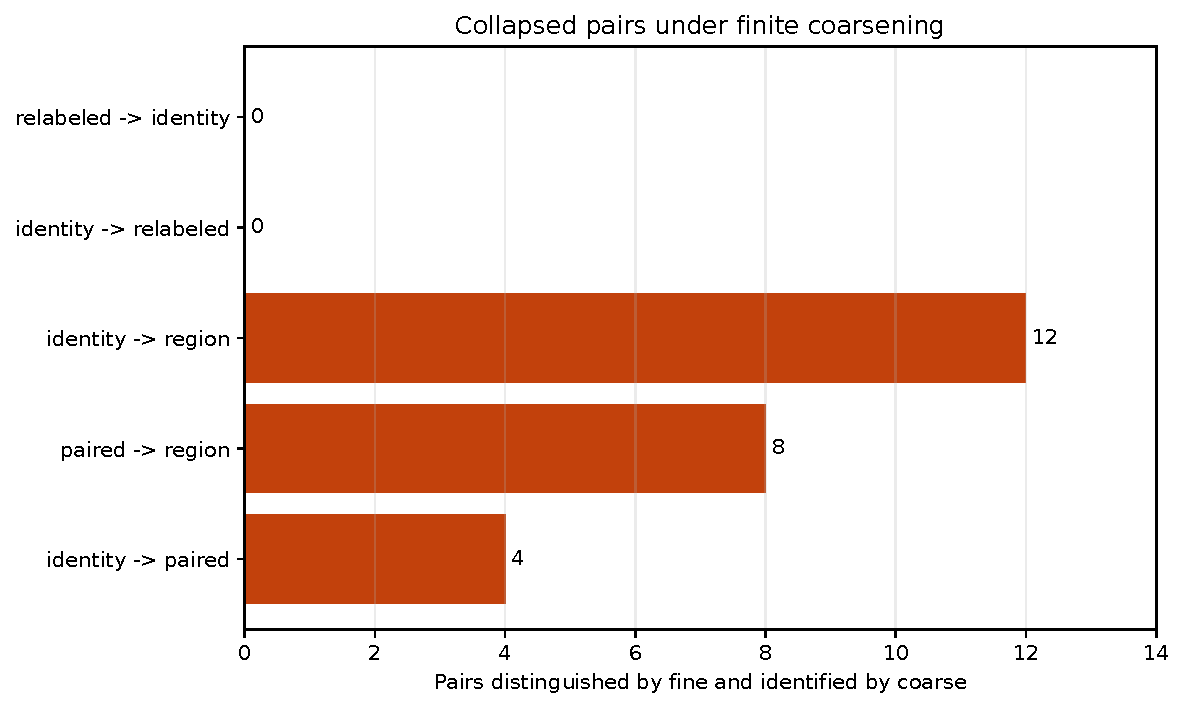
\includegraphics[width=\linewidth]{figures/repo_collapsed_pairs_by_refinement.pdf}
\caption{Collapsed state pairs.}
\label{fig:repo-collapsed}
\end{subfigure}
\caption{Interface refinement results. Strict coarsening reduces the retained quotient classes and identifies world state pairs. Relabeling preserves observational resolution.}
\label{fig:refinementpanel}
\end{figure}

\begin{table}[tbp]
\centering
\caption{Finite interface and refinement summary.}
\label{tab:refinements}
\small
\begin{tabularx}{\textwidth}{@{}Xrrrrcc@{}}
\toprule
Refinement & Fine \(Q\) & Coarse \(Q\) & Collapsed & Strict & Surjective & Injective \\
\midrule
Identity to paired & 8 & 4 & 4 & True & True & False \\
Paired to region & 4 & 2 & 8 & True & True & False \\
Identity to region & 8 & 2 & 12 & True & True & False \\
Identity to relabeled & 8 & 8 & 0 & False & True & True \\
Relabeled to identity & 8 & 8 & 0 & False & True & True \\
\bottomrule
\end{tabularx}
\end{table}

The files \nolinkurl{quotient_maps.csv} and \nolinkurl{collapsed_pairs.csv} contain the 36 entries in the quotient maps and the 24 collapsed pairs, respectively.

\subsection{Validation result}

All eighteen reference tests and eight additional finite checks pass. Each of the twelve regenerated CSV files matches its archived counterpart byte for byte.
